%
%  Peter Vermeer
%  Reference used in this note: "The Arctangent Survival Distribution" by Glen and Leemis
%
\documentclass[12pt,fullpage]{article}
\usepackage{fullpage}
\usepackage{psfrag}                                          % LaTeX graphics tool
\usepackage{pslatex}                                         % avoids the default cmr font
\usepackage{graphicx}                                        % graphics package 
\usepackage{epsfig}                                          % figures
\usepackage{epsfig} 
\usepackage{hyperref}
\usepackage{color}

\begin{document}

\noindent
{\bf Arctangent distribution} (from \color{blue}\url{http://www.math.wm.edu/~leemis/chart/UDR/UDR.html}\color{black})

\noindent
The shorthand $X \sim {\rm arctan}(\lambda, \phi)$ is used to indicate that the
random variable $X$ has the arctangent distribution with phase shift parameter $\phi$ and positive location parameter $\lambda$.
An arctangent random variable $X$ with parameters $\lambda$ and $\phi$ has probability density function 
$$
f(x) = {\frac {\lambda } { \left( \arctan \left( \lambda \,\phi  \right) + 1 / 2 \,\pi  \right)  \left( 1 + {\lambda } ^ {2} \left( x - \phi  \right) ^ {2} \right) }}\qquad \qquad x \geq 0
$$
for
$\lambda > 0$
and
$-\infty < \phi < \infty$.\\
The probability density function with three different choices of parameters is illustrated below.
{\begin{figure}[h!]
\begin{center}
\psfrag{lab1}{$\lambda \kern -0.08 em = \kern -0.08 em  1,\, \phi \kern -0.08 em  = \kern -0.08 em  1$}
\psfrag{lab2}{$\lambda \kern -0.08 em  = \kern -0.08 em  2,\, \phi \kern -0.08 em  = \kern -0.08 em  3$}
\psfrag{lab3}{$\lambda \kern -0.08 em  = \kern -0.08 em  1,\, \phi \kern -0.08 em  = \kern -0.08 em  3$}
\psfrag{labx}{$x$}
\psfrag{labf}{$f(x)$}
\includegraphics[width=3.2in]{ArctangentPlot.ps}
\end{center}
\end{figure}}\\
The cumulative distribution function of $X$ is
$$
F(x) = P(X \le x) = 2 \left( \, {\frac {\arctan \left( \lambda \, \phi  \right) - \arctan \left( -x \lambda + \lambda \, \phi  \right) } {2 \, \arctan \left( \lambda \, \phi  \right) + \pi }} \right) \qquad \qquad x \geq 0.
$$
The survivor function of $X$ is
$$
S(x) = P(X \ge x) = {\frac {\pi + 2 \, \arctan \left( -x\lambda + \lambda \,\phi  \right) }{2 \, \arctan \left( \lambda \, \phi  \right) + \pi }} \qquad \qquad x \geq 0.
$$
The hazard function of $X$ is
$$
h(x) = \frac{f(x)} {S(x)} = {\frac {2 \lambda } { ( 1 + {\lambda } ^ {2} {x} ^ {\kern 0.08 em 2} - 2 \, {\lambda } ^ {2} \phi \, x + {\lambda } ^ {2} {\phi } ^ {\kern 0.04 em 2})  \left( \pi + 2 \, \arctan \left( -x \lambda + \lambda \, \phi  \right)  \right) }} \qquad \qquad x \geq 0.
$$
The cumulative hazard function of $X$ is
$$
H(x) = \ln  \left( 2 \,\arctan \left( \lambda \, \phi  \right) + \pi  \right) - \ln  \left( \pi + 2 \, \arctan \left( \lambda \, \left( -x + \phi  \right)  \right)  \right)   \qquad \qquad x \geq 0.
$$
The inverse distribution function of $X$ is
$$
F ^ {-1}(u) = {\frac {\lambda \, \phi + \tan \left( -\arctan \left( \lambda \, \phi \right) + u \arctan \left( \lambda \, \phi  \right) + 1 / 2 \, u \kern 0.08 em \pi  \right) } {\lambda}} \qquad \qquad 0 < u < 1.
$$
The moments of $X$ are undefined. It follows that the population mean, variance, skewness, and kurtosis of $X$ are also undefined.

\vspace{0.1in}

\noindent
{\bf APPL verification:}
The APPL statements
\begin{verbatim}
X := ArcTanRV(lambda, phi);
CDF(X);
SF(X);
HF(X);
IDF(X);
Mean(X);
Variance(X);
Skewness(X);
Kurtosis(X);
MGF(X);
\end{verbatim}
verify the cumulative distribution function, survivor function, hazard function, population mean, variance, skewness, kurtosis, and moment generating function.
\end{document}
